\mbox{$\displaystyle $\,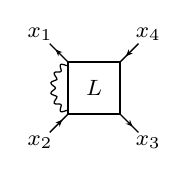
\begin{tikzpicture}[x=0.550cm, y=0.550cm, line width=0.450pt, baseline={([yshift=-0.6ex]0,0)}]
  \draw plot[smooth, tension=0.7] coordinates {(-0.600,0.600) (-0.602,0.551) (-0.615,0.522) (-0.646,0.521) (-0.693,0.537) (-0.741,0.550) (-0.775,0.543) (-0.784,0.509) (-0.774,0.460) (-0.760,0.413) (-0.763,0.382) (-0.792,0.371) (-0.842,0.371) (-0.892,0.368) (-0.921,0.350) (-0.919,0.316) (-0.894,0.272) (-0.866,0.232) (-0.859,0.201) (-0.883,0.182) (-0.930,0.166) (-0.976,0.147) (-0.998,0.121) (-0.986,0.089) (-0.948,0.056) (-0.908,0.026) (-0.892,0.000) (-0.908,-0.026) (-0.948,-0.056) (-0.986,-0.089) (-0.998,-0.121) (-0.976,-0.147) (-0.930,-0.166) (-0.883,-0.182) (-0.859,-0.201) (-0.866,-0.232) (-0.894,-0.272) (-0.919,-0.316) (-0.921,-0.350) (-0.892,-0.368) (-0.842,-0.371) (-0.792,-0.371) (-0.763,-0.382) (-0.760,-0.413) (-0.774,-0.460) (-0.784,-0.509) (-0.775,-0.543) (-0.741,-0.550) (-0.693,-0.537) (-0.646,-0.521) (-0.615,-0.522) (-0.602,-0.551) (-0.600,-0.600)};
  \draw (0.000,0.000) -- (-0.600,0.600);
  \draw (0.000,0.000) -- (-0.600,-0.600);
  \draw (0.000,0.000) -- (0.600,-0.600);
  \draw (0.000,0.000) -- (0.600,0.600);
  \draw (-0.600,0.600) -- (-1.024,1.024);
  \fill (-0.889,0.889) -- (-0.825,0.730) -- (-0.814,0.814) -- (-0.730,0.825) -- cycle;
  \draw (-0.600,-0.600) -- (-1.024,-1.024);
  \fill (-0.735,-0.735) -- (-0.895,-0.799) -- (-0.810,-0.810) -- (-0.799,-0.895) -- cycle;
  \draw (0.600,-0.600) -- (1.024,-1.024);
  \fill (0.889,-0.889) -- (0.825,-0.730) -- (0.814,-0.814) -- (0.730,-0.825) -- cycle;
  \draw (0.600,0.600) -- (1.024,1.024);
  \fill (0.735,0.735) -- (0.895,0.799) -- (0.810,0.810) -- (0.799,0.895) -- cycle;
  \fill[white] (-0.600,-0.600) rectangle (0.600,0.600);
  \draw (-0.600,-0.600) rectangle (0.600,0.600);
  \node[font=\footnotesize, inner sep=0.6pt] at (0.000,0.000) {$L$};
  \node[font=\footnotesize, inner sep=0pt, anchor=315] at (-1.088,1.088) {$x_{1}$};
  \node[font=\footnotesize, inner sep=0pt, anchor=45] at (-1.088,-1.088) {$x_{2}$};
  \node[font=\footnotesize, inner sep=0pt, anchor=135] at (1.088,-1.088) {$x_{3}$};
  \node[font=\footnotesize, inner sep=0pt, anchor=225] at (1.088,1.088) {$x_{4}$};
\end{tikzpicture}}
\diagramgap
\mbox{$\displaystyle -\,$\,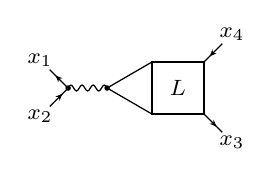
\begin{tikzpicture}[x=0.550cm, y=0.550cm, line width=0.450pt, baseline={([yshift=-0.6ex]0,0)}]
  \draw plot[smooth, tension=0.7] coordinates {(-2.535,0.000) (-2.503,0.049) (-2.471,0.069) (-2.439,0.049) (-2.406,0.000) (-2.374,-0.049) (-2.342,-0.069) (-2.310,-0.049) (-2.278,0.000) (-2.246,0.049) (-2.214,0.069) (-2.181,0.049) (-2.149,0.000) (-2.117,-0.049) (-2.085,-0.069) (-2.053,-0.049) (-2.021,0.000) (-1.989,0.049) (-1.956,0.069) (-1.924,0.049) (-1.892,0.000) (-1.860,-0.049) (-1.828,-0.069) (-1.796,-0.049) (-1.764,0.000) (-1.731,0.049) (-1.699,0.069) (-1.667,0.049) (-1.635,0.000)};
  \draw (-0.600,0.600) -- (-1.635,0.000);
  \draw (-0.600,-0.600) -- (-1.635,0.000);
  \draw (0.000,0.000) -- (0.600,-0.600);
  \draw (0.000,0.000) -- (0.600,0.600);
  \draw (-2.535,0.000) -- (-2.959,0.424);
  \fill (-2.824,0.289) -- (-2.760,0.130) -- (-2.749,0.214) -- (-2.665,0.225) -- cycle;
  \draw (-2.535,0.000) -- (-2.959,-0.424);
  \fill (-2.670,-0.135) -- (-2.830,-0.199) -- (-2.745,-0.210) -- (-2.734,-0.295) -- cycle;
  \draw (0.600,-0.600) -- (1.024,-1.024);
  \fill (0.889,-0.889) -- (0.825,-0.730) -- (0.814,-0.814) -- (0.730,-0.825) -- cycle;
  \draw (0.600,0.600) -- (1.024,1.024);
  \fill (0.735,0.735) -- (0.895,0.799) -- (0.810,0.810) -- (0.799,0.895) -- cycle;
  \fill[white] (-0.600,-0.600) rectangle (0.600,0.600);
  \draw (-0.600,-0.600) rectangle (0.600,0.600);
  \node[font=\footnotesize, inner sep=0.6pt] at (0.000,0.000) {$L$};
  \fill (-2.535,0.000) circle (0.064);
  \fill (-1.635,0.000) circle (0.064);
  \node[font=\footnotesize, inner sep=0pt, anchor=315] at (-3.023,0.488) {$x_{1}$};
  \node[font=\footnotesize, inner sep=0pt, anchor=45] at (-3.023,-0.488) {$x_{2}$};
  \node[font=\footnotesize, inner sep=0pt, anchor=135] at (1.088,-1.088) {$x_{3}$};
  \node[font=\footnotesize, inner sep=0pt, anchor=225] at (1.088,1.088) {$x_{4}$};
\end{tikzpicture}}
